%%%%%%%%%%%%%%%%%%%%%%%%%%% asme2e.tex %%%%%%%%%%%%%%%%%%%%%%%%%%%%%%%
% Template for producing ASME-format articles using LaTeX            %
% Written by   Harry H. Cheng                                        %
%              Integration Engineering Laboratory                    %
%              Department of Mechanical and Aeronautical Engineering %
%              University of California                              %
%              Davis, CA 95616                                       %
%              Tel: (530) 752-5020 (office)                          %
%                   (530) 752-1028 (lab)                             %
%              Fax: (530) 752-4158                                   %
%              Email: hhcheng@ucdavis.edu                            %
%              WWW:   http://iel.ucdavis.edu/people/cheng.html       %
%              May 7, 1994                                           %
% Modified: February 16, 2001 by Harry H. Cheng                      %
% Modified: January  01, 2003 by Geoffrey R. Shiflett                %
% Use at your own risk, send complaints to /dev/null                 %
%%%%%%%%%%%%%%%%%%%%%%%%%%%%%%%%%%%%%%%%%%%%%%%%%%%%%%%%%%%%%%%%%%%%%%

%%% use twocolumn and 10pt options with the asme2e format
\documentclass[cleanfoot,cleanhead,onecolumn,10pt,notitlepage]{asme2e}
\special{papersize=8.5in,11in}

\usepackage{listings}
\usepackage{graphicx}
\usepackage{amsmath}
\lstset{
    breaklines=true, % break lines for files
    basicstyle=\scriptsize,
    numbers=left,
    showstringspaces=false,
    frame=l
}

%% The class has several options
%  onecolumn/twocolumn - format for one or two columns per page
%  10pt/11pt/12pt - use 10, 11, or 12 point font
%  oneside/twoside - format for oneside/twosided printing
%  final/draft - format for final/draft copy
%  cleanfoot - take out copyright info in footer leave page number
%  cleanhead - take out the conference banner on the title page
%  titlepage/notitlepage - put in titlepage or leave out titlepage
%  
%% The default is oneside, onecolumn, 10pt, final

%%% You need to remove 'DRAFT: ' in the title for the final submitted version.
\title{Computer Project \#3}

%%% first author
\author{Shaun Harris
    \affiliation{
	Department of Mechanical and Aerospace Engineering\\
	Utah State University \\
    Email: shaun.r.harris@gmail.com
    }
}


\begin{document}

\maketitle 



%%%%%%%%%%%%%%%%%%%%%%%%%%%%%%%%%%%%%%%%%%%%%%%%%%%%%%%%%%%%%%%%%%%%%%

\begin{abstract}
    {\it A staggard grid Navier-Stokes solver is implemented to solve a driven cavity problem, and a channel flow problem.  The Pressure, u-velocity and v-velocity are all staggard and solved for separatley.  The necessary equations and the implemented code is provided in this paper.}
\end{abstract}

%%%%%%%%%%%%%%%%%%%%%%%%%%%%%%%%%%%%%%%%%%%%%%%%%%%%%%%%%%%%%%%%%%%%%%

\begin{nomenclature}
\entry{$u$}{Velocity in the x-direction}
\entry{$v$}{Velocity in the y-direction}
\entry{$P$}{Pressure}
\entry{$a_{i,j}$}{Coefficient for final discretized equation referencing neighbor $i (N,E,S,W,P)$ on $j (u,v,P)$ mesh}
\entry{$\tilde{a}_{P,j}$}{Coefficient for final discretized equation referencing center $P$ on $j (u,v,P)$ mesh and divided by $\Omega$ correction factor}
\entry{$\Omega$}{non-linear correction factor for momentum equations}
\entry{$\Omega_P$}{linear correction factor for pressure equation}
\entry{$\alpha$}{Pressure blending factor}
\end{nomenclature}

%%%%%%%%%%%%%%%%%%%%%%%%%%%%%%%%%%%%%%%%%%%%%%%%%%%%%%%%%%%%%%%%%%%%%%

\tableofcontents   

\section{INTRODUCTION}

In order to solve using this method, a staggered grid was utilized.  Fig. \ref{fig:stencil} shows how the $u,v,$ and $P$ values were saved on the grid.  The momentum equation is discretized from Eq. \ref{eq:umom} to \ref{eq:disumom}

\begin{equation}
\begin{aligned}
\frac{\partial (\rho u u)}{\partial x} + \frac{\partial (\rho v u)}{\partial y} &=
-\frac{\partial P}{\partial x} 
+ \frac{\partial }{\partial x} \left( \mu \frac{\partial u}{\partial x} \right)
+ \frac{\partial }{\partial y} \left( \mu \frac{\partial u}{\partial y} \right)
+ \frac{\partial }{\partial x} \left( \mu \frac{\partial u}{\partial x} \right)
+ \frac{\partial }{\partial y} \left( \mu \frac{\partial v}{\partial y} \right)
\label{eq:umom}
\end{aligned}
\end{equation}

%%%%%%%%%%%%%%%%%%%%%%%%%%%%%%%%%%%%%%%%%%%%%%%%%%%%%%%%%%%%%%%%%%%%%%

\section{NUMERICAL METHOD}




%%%%%%%%%%%%%%%%%%%%%%%%%%%%%%%%%%%%%%%%%%%%%%%%%%%%%%%%%%%%%%%%%%%%%%

\section{RESULTS}


%%%%%%%%%%%%%%%%%%%%%%%%%%%%%%%%%%%%%%%%%%%%%%%%%%%%%%%%%%%%%%%%%%%%%%

\section{CONCLUSION}



%%%%%%%%%%%%%%%%%%%%%%%%%%%%%%%%%%%%%%%%%%%%%%%%%%%%%%%%%%%%%%%%%%%%%%

%\bibliographystyle{asmems4}
%\bibliography{asme2e}

%%%%%%%%%%%%%%%%%%%%%%%%%%%%%%%%%%%%%%%%%%%%%%%%%%%%%%%%%%%%%%%%%%%%%%

%\section*{FIGURES}

\begin{figure}[t]
\begin{center}
    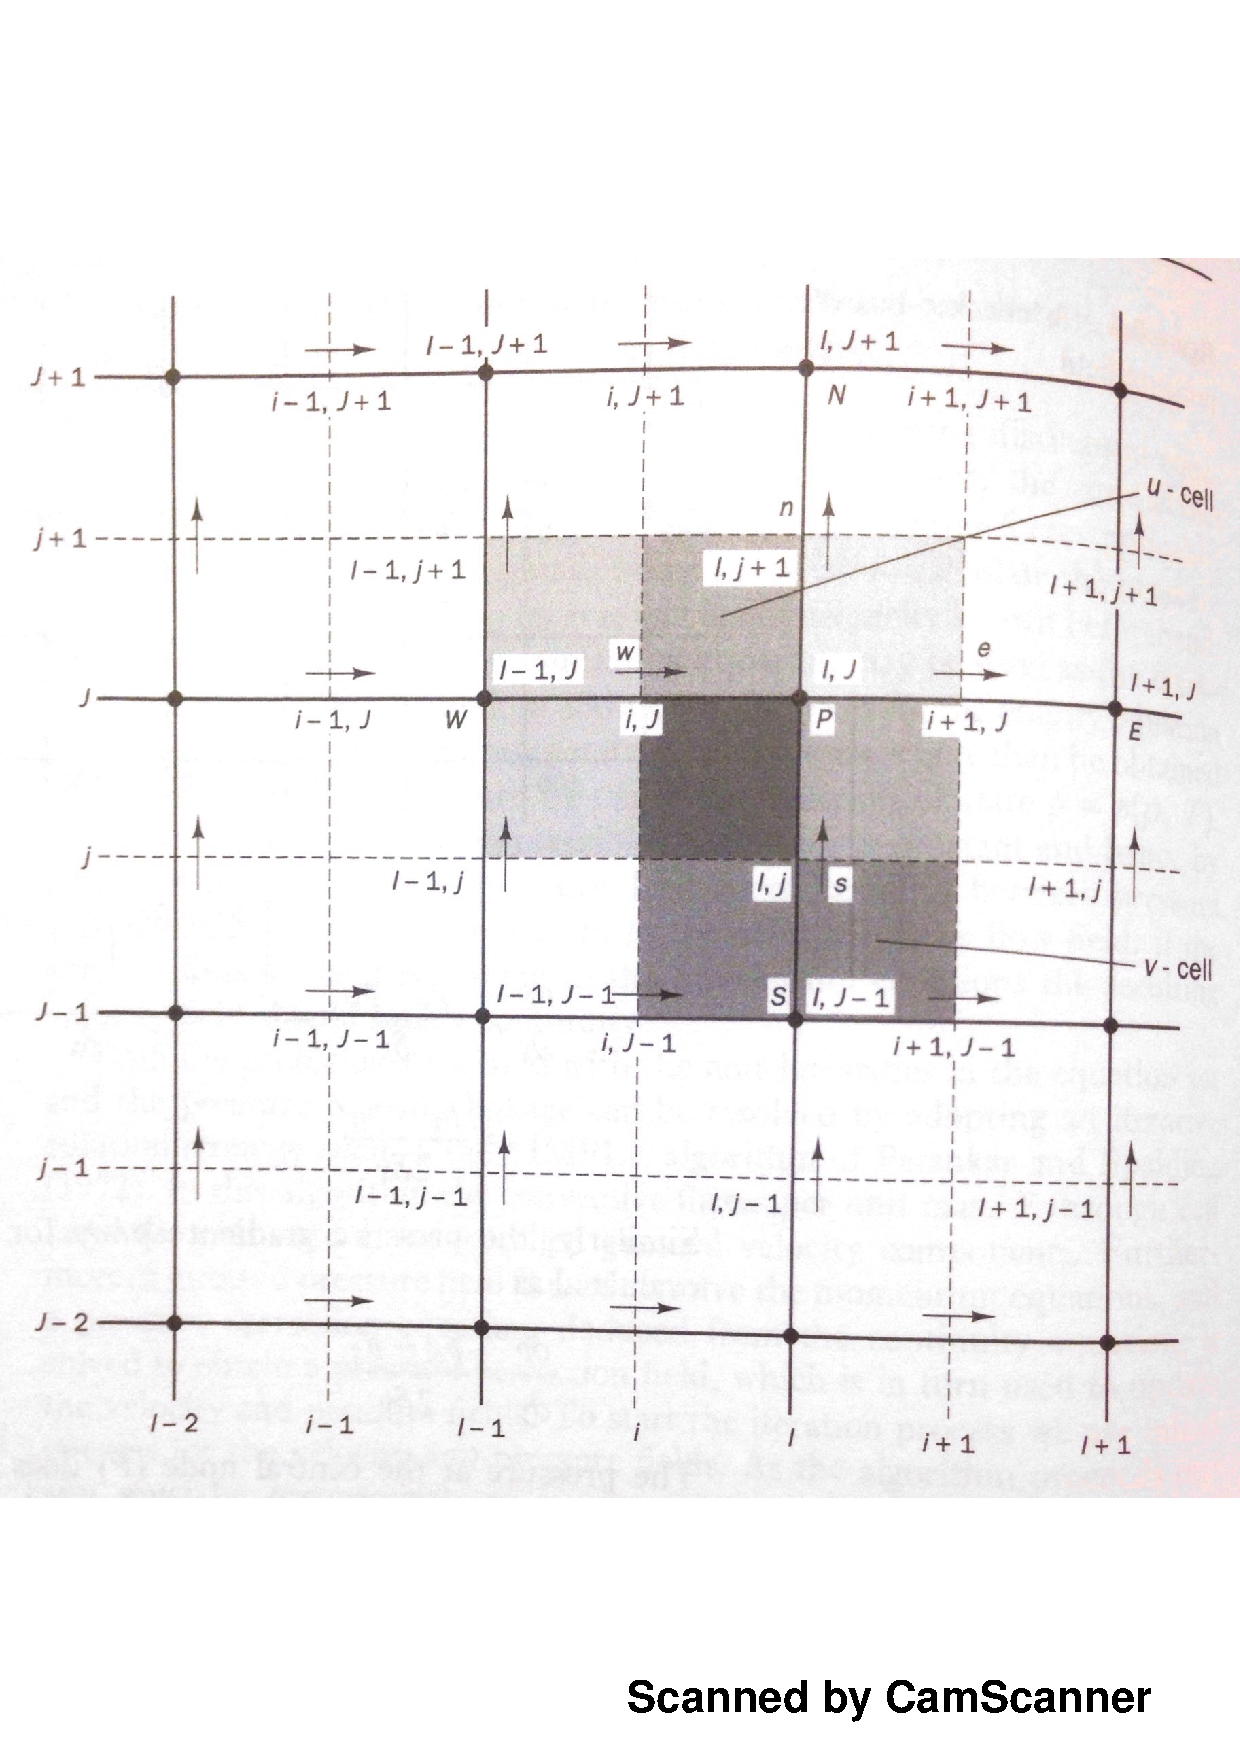
\includegraphics[width=0.4\linewidth]{Stencil.pdf}
    \caption{REPRESENTATION OF STENCIL FOR GRID GENERATION}
    \label{fig:stencil}
\end{center}
\end{figure}

%%%%%%%%%%%%%%%%%%%%%%%%%%%%%%%%%%%%%%%%%%%%%%%%%%%%%%%%%%%%%%%%%%%%%%
\clearpage

\appendix

\section{Code}

\subsection{Subroutines}
\lstinputlisting[language=Fortran]{../Project3_code/Types.f90}
\subsection{Main program}
\lstinputlisting[language=Fortran]{../Project3_code/Project3.f90}



\end{document}
